\documentclass[xcolor={dvipsnames,table}]{beamer}
\usecolortheme[named=PineGreen]{structure} 
\usetheme{Warsaw}
\pdfpageattr {/Group << /S /Transparency /I true /CS /DeviceRGB>>}
\usepackage{hyperref}
\usepackage{graphicx}
\usepackage{aas_macros}
\usepackage{array}




\setbeamertemplate{caption}{\raggedright\insertcaption\par}
  \setbeamertemplate{enumerate items}[default]
  \setbeamertemplate{itemize items}{$\sim$}
  
  \AtBeginSection[]{
  	\begin{frame}
  		\vfill
  		\centering
  		\begin{beamercolorbox}[sep=18pt,center,shadow=true,rounded=true]{title}
  			\usebeamerfont{title}\secname\par%
  		\end{beamercolorbox}
  		\vfill
  	\end{frame}
  }
  
  
  \newcommand{\subheader}{    		\begin{center}
  	\begin{beamercolorbox}[sep=4pt,center,shadow=true,rounded=true]{title}
  		\usebeamerfont{title}\subsecname\par%
  	\end{beamercolorbox}
  	\vfill
  	\end{center}}


\newcommand{\req}{\ensuremath{\rho_{eq}}} %Since it's used so often. ensuremath lets it be used in equations or text
\newcommand{\dst}{\ensuremath{D_{st}}} %Now I'm just getting lazy. 
\newcommand{\f}{\ensuremath{F_{10.7}}} %Because latex doesn't allow numbers in commands
\newcolumntype{C}{>{$}c<{$}} %To enable math mode in tables (for saying things like B_z)

\begin{document}
\title[Statistical Modeling of Earth's Plasmasphere]{Statistical Modeling of Earth's Plasmasphere}
\author{Victoir Veibell}
\date{July 21, 2016}
\setbeamertemplate{navigation symbols}{}

\begin{frame}
\titlepage
\end{frame}



%%%%%%%%%%%%%%%%%%%%%%%%%%%%%%%%%%%%%%%%%%%%%%%%%%%
%  _____      _                 _            _   _             
% |_   _|    | |               | |          | | (_)            
%   | | _ __ | |_ _ __ ___   __| |_   _  ___| |_ _  ___  _ __  
%   | || '_ \| __| '__/ _ \ / _` | | | |/ __| __| |/ _ \| '_ \ 
%   | || | | | |_| | | (_) | (_| | |_| | (__| |_| | (_) | | | |
%  |___|_| |_|\__|_|  \___/ \__,_|\__,_|\___|\__|_|\___/|_| |_|
%%%%%%%%%%%%%%%%%%%%%%%%%%%%%%%%%%%%%%%%%%%%%%%%%%%
\section{Introduction}

\subsection{System}
\begin{frame} 
	
\begin{figure}[htp]
	\centering
	\includegraphics[scale=0.35]{{Figures/MagnetoOverview.jpg}}
	\caption{Overview of the magnetosphere and plasmasphere \cite{MagnetosphereOverallFigure}.}
	\label{RingCurrentFigure}
\end{figure}

\end{frame}

\begin{frame}
	\begin{figure}[htp]
		\centering
		\includegraphics[scale=0.2]{{Figures/innermag-2.jpg}}
		\caption{Overview of inner magnetosphere. Adapted from \cite{InnerMagNASA}.}
		\label{fig:magnetosphereoverview}
	\end{figure}
\end{frame}


\begin{frame}
	\begin{figure}[htp]
		\centering
		\includegraphics[scale=0.12]{{Figures/magnetosphere.jpg}}
		\caption{Currents in/around the magnetosphere. Adapted from \cite{MagnetosphereCurrentFigure}.}
		\label{RingCurrentFigure}
	\end{figure}
\end{frame}



%%%%%%%%%%%%%%%%%%%%%%%%%%%%%%%%%%%%%%%%%%%%%%%%%%%
%___  ___      _   _            _   _             
%|  \/  |     | | (_)          | | (_)            
%| .  . | ___ | |_ ___   ____ _| |_ _  ___  _ __  
%| |\/| |/ _ \| __| \ \ / / _` | __| |/ _ \| '_ \ 
%| |  | | (_) | |_| |\ V | (_| | |_| | (_) | | | |
%\_|  |_/\___/ \__|_| \_/ \__,_|\__|_|\___/|_| |_|
%%%%%%%%%%%%%%%%%%%%%%%%%%%%%%%%%%%%%%%%%%%%%%%%%%%
\subsection{Motivation}
\begin{frame}
	\begin{figure}
		\centering
		\includegraphics[width=0.75\linewidth]{Figures/TE_space_weather_diagram}
		\caption{Impacts of Space Weather [Lanzerotti]}
		\label{fig:TE_space_weather_diagram}
	\end{figure}
\end{frame}




\subsection{Data}

\begin{frame}
	\subheader
	Data come from three sources:
	\small
	\begin{itemize}
		\item Denton (2007) for \req, MLT, and $AE$ \\
		\item King (2005) for \f
		\item Kondrashov (2014) for $B_z$, $V_{SW}$, Kp, $\rho_{sw}$, and $D_{st}$ \\
	\end{itemize}
\end{frame}

\begin{frame}
	Data coverage:
	\begin{itemize}
		\item Denton (2007): 10 minute, non-uniform, non-complete, from 1980-1991, GOES 2, 5, 6, and 7
		\item King (2005): 1 hour uniform, non-complete, from 1972-2013
		\item Kondrashov (2014): 1 hour uniform, complete, from 1972-2013
	\end{itemize}
\end{frame}


\begin{frame}
	\begin{figure}[htp!]
		\centering
		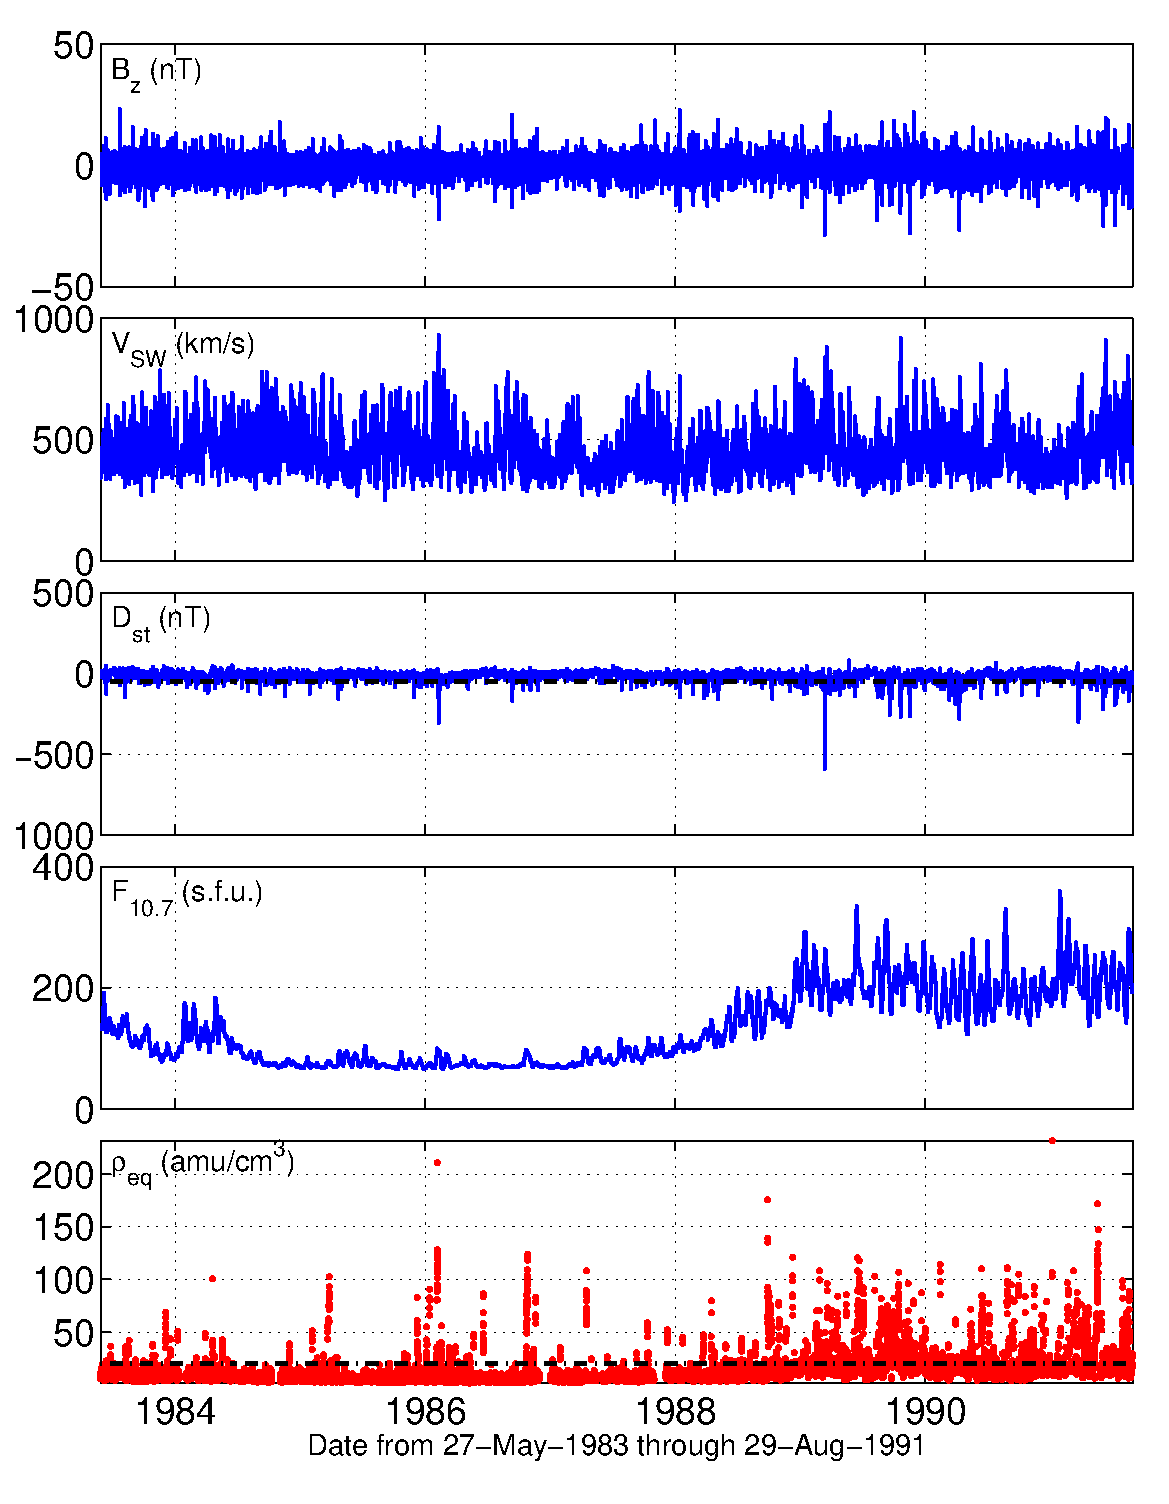
\includegraphics[width=0.5\linewidth]{Figures/alldata-GOES6-1983-1991}
		\caption{Data coverage with dashed lines indicating default event thresholds.}
		\label{fig:alldata-GOES6-1983-1991}
	\end{figure}
\end{frame}

\begin{frame}
	\req\ is derived from toroidal harmonic frequencies in plasmatrough. Harmonics are not always detectable.
	\begin{figure}[htp!]
		\centering
		\includegraphics[width=0.4\linewidth]{Figures/Takahashi2010Availability.png}
		\includegraphics[width=0.4\linewidth]{Figures/databyMLT}
		\caption{Left: Detection rate of $f_{T3\_30m}$ for magnetic latitudes of 5, 9, and 11 degrees (curves A, B, and C respectively) [Takahashi (2010)]. Right: MLT of all available data.}
		\label{fig:Takahashi2010Availability}
	\end{figure}
\end{frame}

\begin{frame}
\begin{figure}[htp!]
	\centering
	\includegraphics[width=0.5\linewidth]{Figures/alldata-GOES6-10Mar1989-17Mar1989.eps}%alldata-GOES6-1989-1989}
	\caption{Data from GOES 6 around March 1989 geomagnetic storm.}
	\label{fig:alldata-GOES6-1989-1989}
\end{figure}
\end{frame}

\begin{frame}
	\begin{figure}[htp]
		\centering
		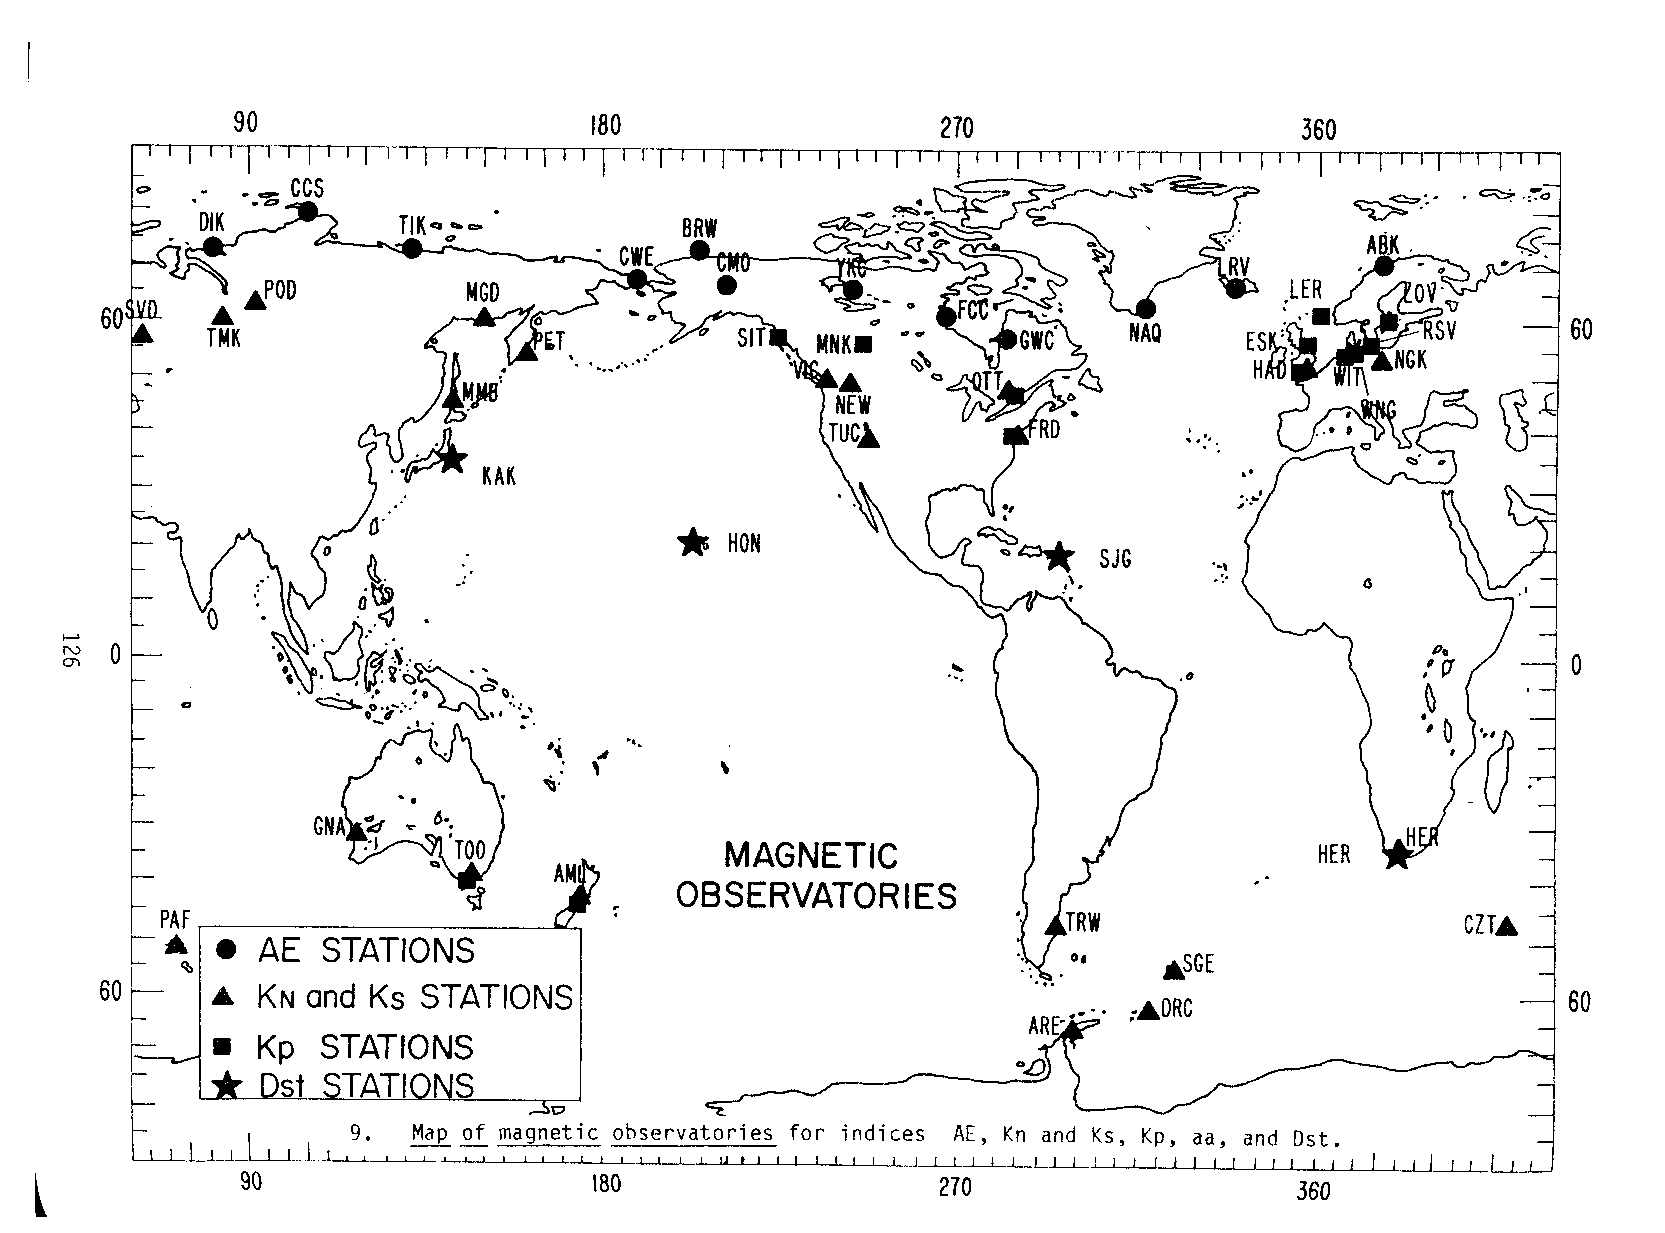
\includegraphics[scale=0.35]{{Figures/StationMap.eps}}
		\caption{Map of ground stations used to measure the $K_p$, $AE$, and \dst\ indices \cite{CommonMagneticIndices}.}
		\label{fig:GroundStations}
	\end{figure}
\end{frame}



\begin{frame}
	\begin{figure}[htp!]
		\centering
		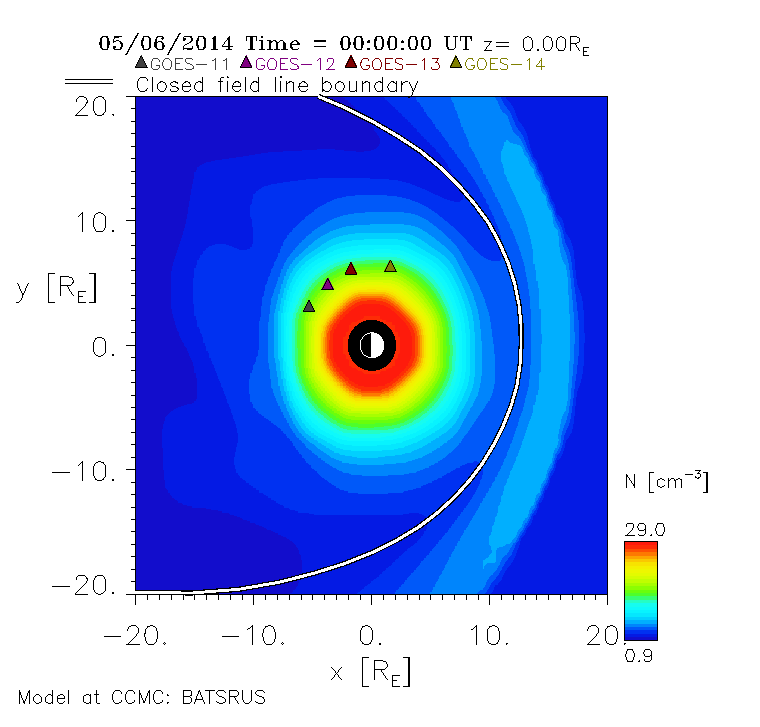
\includegraphics[width=0.45\linewidth]{Figures/idl_798387073825_050215_2_20140506_000000_before}
		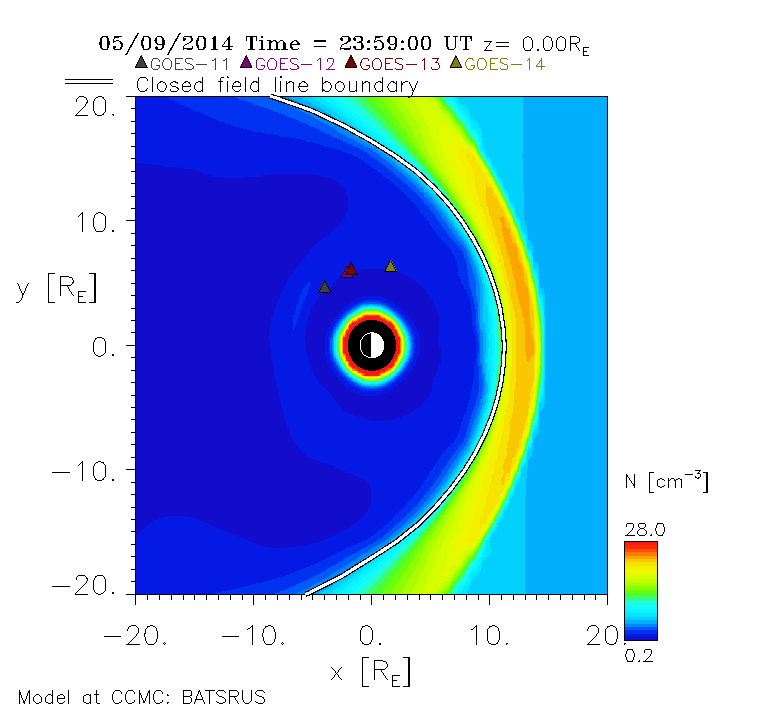
\includegraphics[width=0.45\linewidth]{Figures/idl_798605093993_050215_2_20140509_235900_after}
		\caption{Model of magnetopause/plasmasphere before and after geomagnetic activity, showing location of GOES satellites in geosynchronous orbit \cite{CCMC}.}
		\label{fig:PlasmapauseLocation}
	\end{figure}
\end{frame}

%http://iswa.ccmc.gsfc.nasa.gov/IswaSystemWebApp/index.jsp?i_1=1&l_1=18&t_1=152&w_1=500&h_1=400&s_1=2014-05-09%2021:34:36.0_0_10_3&i_2=41&l_2=47&t_2=607&w_2=542&h_2=481&s_2=2014-05-09%2021:57:48.0_0_10_3&i_3=44&l_3=591&t_3=780&w_3=500&h_3=333&s_3=2014-05-09%2021:49:48.0_0_10_3&i_4=335&l_4=1094&t_4=725&w_4=800&h_4=400&s_4=2014-05-09%2019:30:00.0!3!&i_5=39&l_5=1370&t_5=325&w_5=500&h_5=333&s_5=2014-05-09%2021:49:48.0_0_10_3&i_6=443&l_6=597&t_6=121&w_6=720&h_6=586&s_6=2014-05-09%2021:58:00.0_0_10_3

%http://ccmc.gsfc.nasa.gov/results/viewrun.php?domain=GM&runnumber=Lois_Smith_050215_2

\begin{frame}
	\begin{figure}[htp!]
		\centering
		\includegraphics[width=0.9\linewidth]{Figures/PlasmapauseLocation.png}
		\caption{Model of plasmapause location as it varies with geomagnetic activity where the symbols indicate the local time of maximum plasmapause location \cite{OBrien2003EmpiricalPlasmapause}.}
		\label{fig:PlasmapauseLocation}
	\end{figure}
\end{frame}

\begin{frame}
	\begin{figure}[htp]
		\centering
		\includegraphics[scale=0.2]{{Figures/LemairePlasmapauseKnee.png}}
		\caption{Plasmapause position varying with $K_p$ as represented by several particular plasmapause crossings made on outbound passes between local times of midnight and 0400 \cite{LemaireEarthsPlasmasphere}.}
		\label{fig:LemaireKnee}
	\end{figure}
\end{frame}


\section{Methodology}
\begin{frame}
Three main methods of analysis used:
\begin{enumerate}
	\item Linear/Auto-Regressive with exogenous inputs (ARX) 
	\item Nonlinear Neural Network
	\item Epoch
\end{enumerate}
\end{frame}

\subsection{Linear and ARX}

\begin{frame}
\subheader
	Start with Box-Jenkins model:
	\begin{align*}
	x(t)&=\sum_{j=1}^{m}{b_j \cdot f(t-j\Delta t)}+c + \varepsilon_t
	\end{align*}
	Modified to be an autoregressive model with exogenous inputs (ARX):
	\begin{align*}
	\hat{x}(t)&=\sum_{i=1}^la_i\cdot x(t-i\Delta t)+\sum_{j=1}^m b_j\cdot f(t-j\Delta t)+c+\varepsilon_t
	\label{ARXEqn}
	\end{align*}
\end{frame}


\begin{frame}
	Resultant matrix to solve:
        \[
        \left( \begin{array}{ccccccc}
        x_0 & ... & x_{\tau-1} & f_0 & ... & f_{\tau-1} & 1\\
        x_1 &     & x_\tau & f_\tau &  &f_\tau & 1\\
        ... &     &     &     &  &   & \\
        x_{N-\tau} & ... & x_{N-1} & f_{N-\tau} & ... & f_{N-1} & 1
        \end{array} \right)
        \left(\begin{array}{c}
        a_0\\...\\a_{\tau-1}\\b_0\\...\\b_{\tau-1}\\c
        \end{array}\right)
        =
        \left(                                                                                                                                                                                    
        \begin{array}{c}
        x_\tau \\ x_{\tau+1} \\ ... \\ x_{N}
        \end{array}
        \right)
        \]
\end{frame}

\begin{frame}
	\begin{figure}[htp]
		\centering
		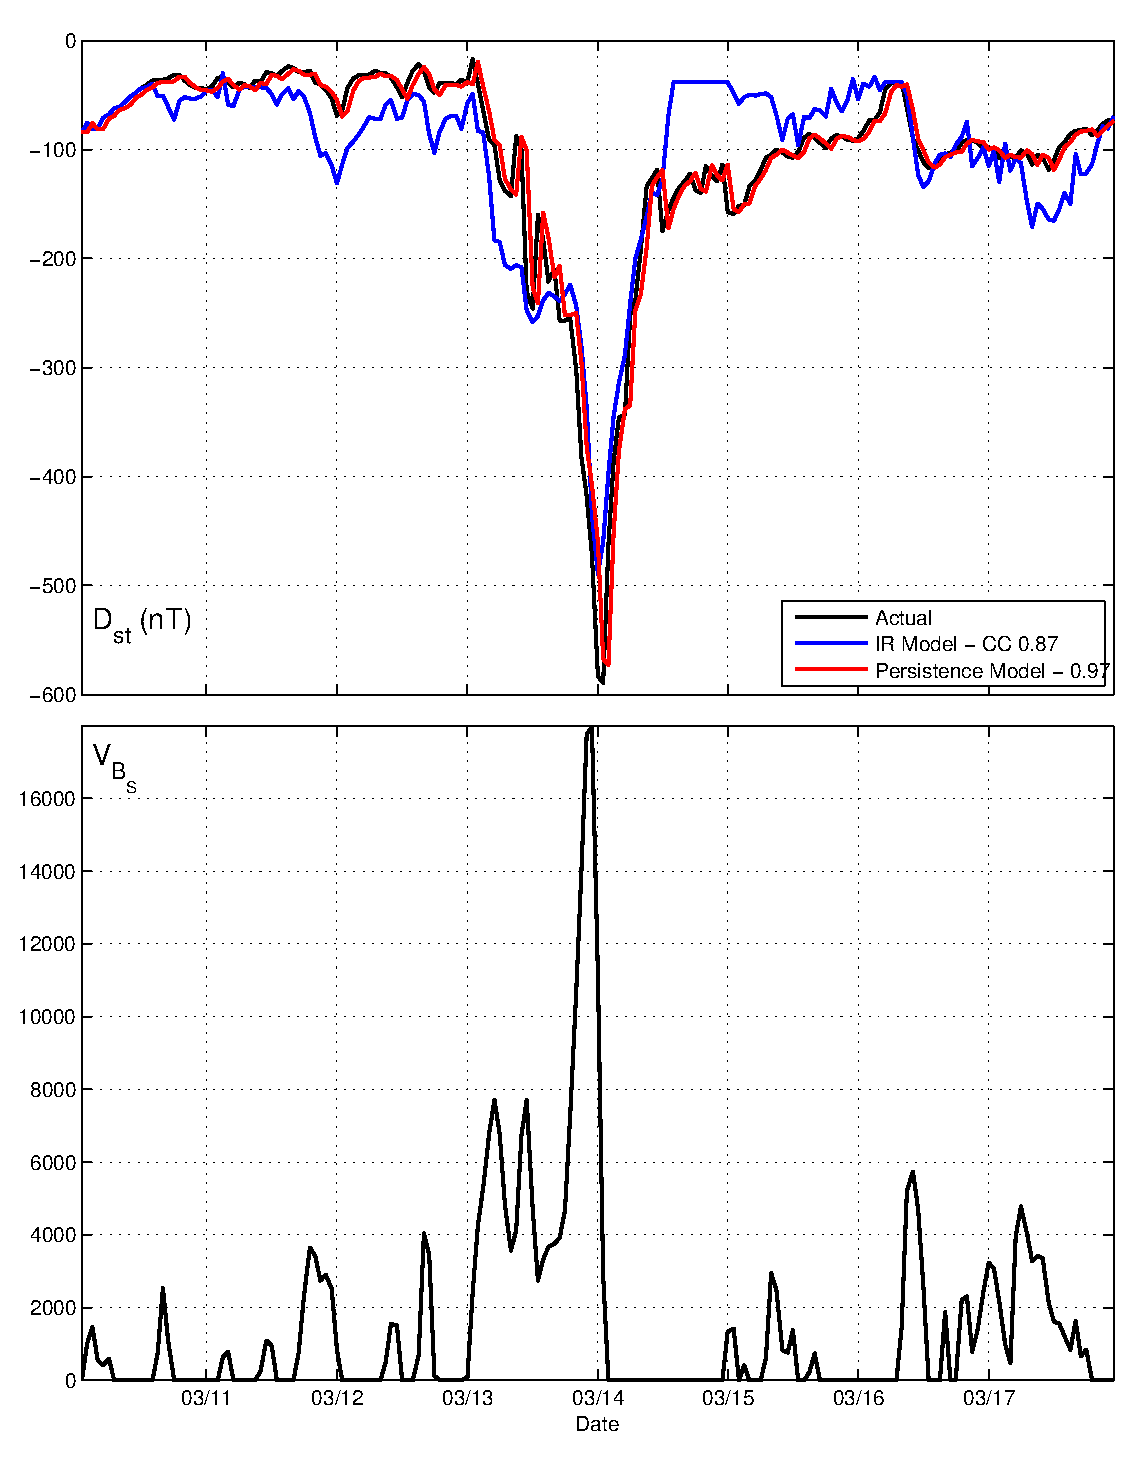
\includegraphics[scale=0.25]{{Figures/BasicModelExample-GOES6}}
		\caption{Top: \dst\ (black), persistence (red), 12-hour impulse response model (blue). Bottom: $vB_S$ input.}
		\label{VBzIRplot}
	\end{figure}
\end{frame}


\subsection{Neural Network}

\begin{frame}
	\subheader
	Neural Network model benefits:
	\begin{enumerate}
		\item Can model nonlinear effects
		\item 
	\end{enumerate}
	Neural Network model disadvantages:
	\begin{enumerate}
		\item Susceptible to overfitting
		\item More complex to create and analyze
		\item No closed-form optimum solution
	\end{enumerate}
\end{frame}


\begin{frame}
	\begin{figure}[htp!]
		\centering
		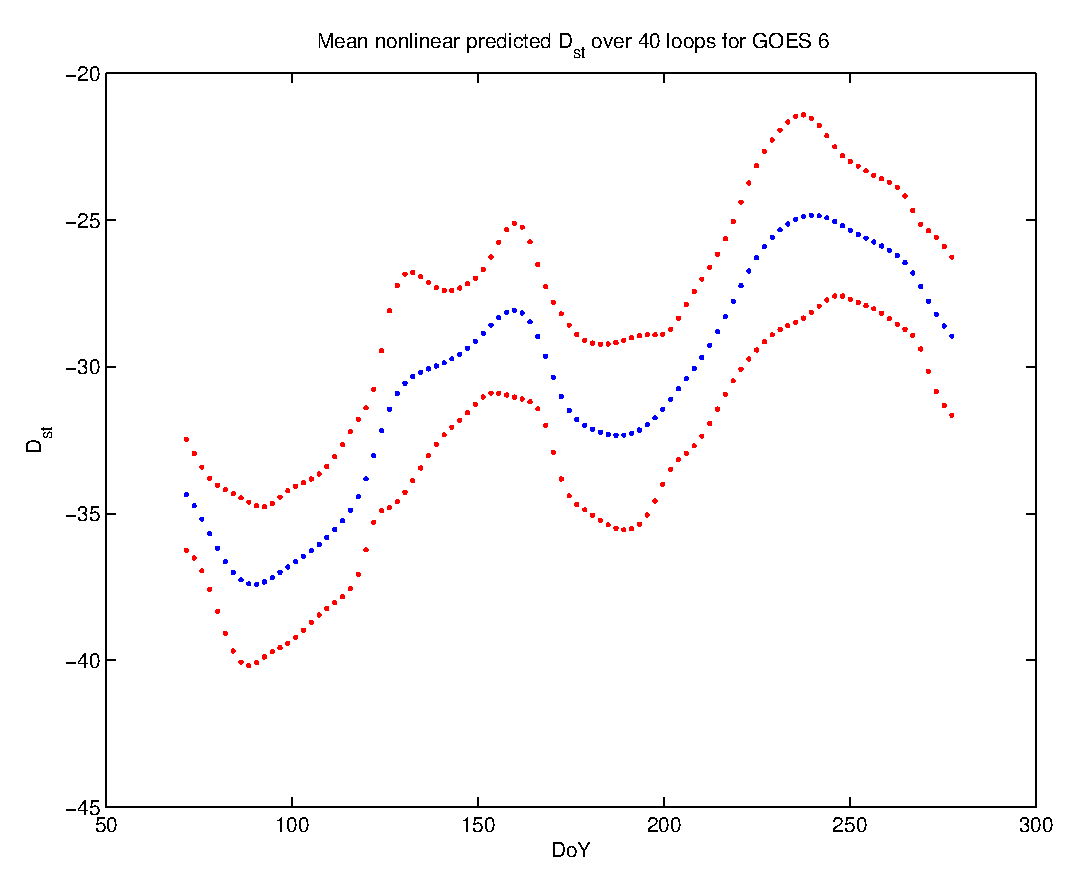
\includegraphics[width=0.7\linewidth]{Figures/NNDoY-Dst-GOES6}	
		\caption{\dst\ predicted by nonlinear model of day of year.}
		\label{fig:DoYDst}
	\end{figure}
\end{frame}




\subsection{Epoch}
\begin{frame}
	\subheader
	Epoch Analysis averages multiple events to find patterns.
\begin{figure}
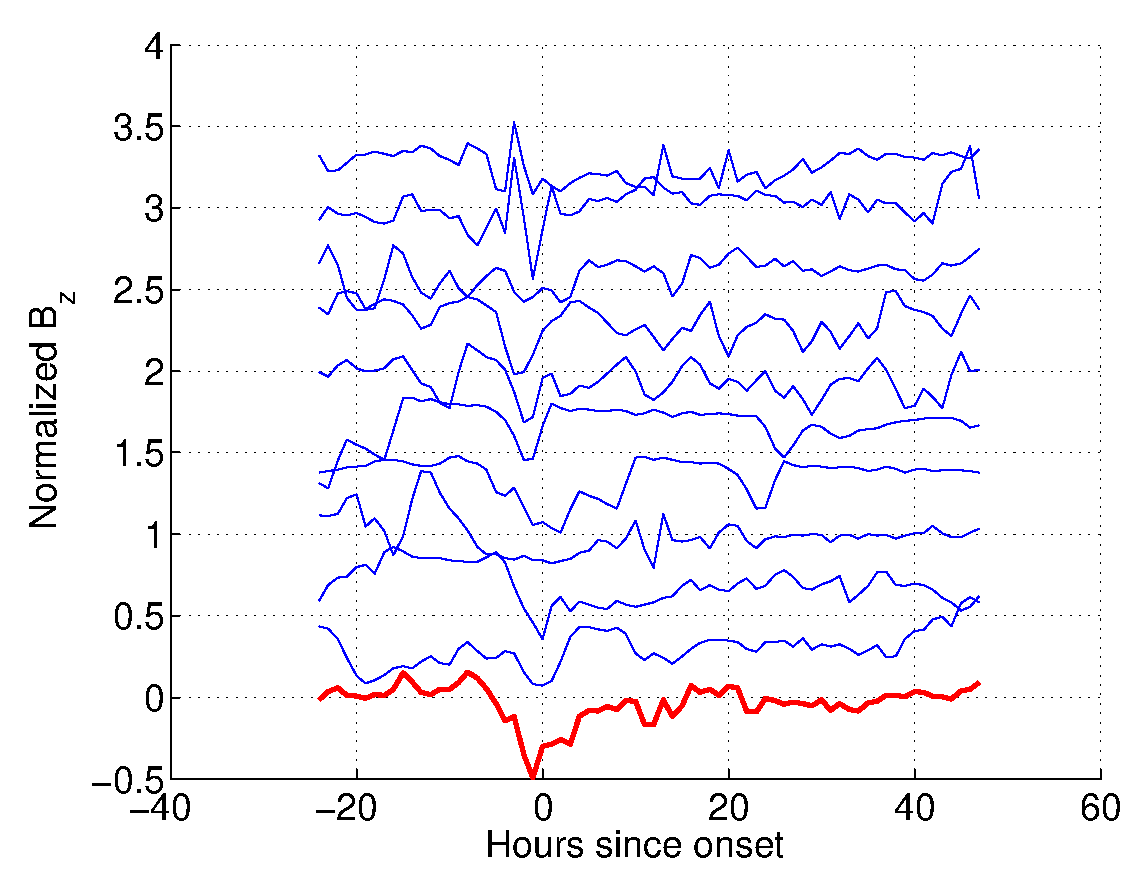
\includegraphics[scale=0.35]{Figures/epochexample}
\caption{Sample epoch of first ten events and median}
\label{fig:epochexample}
\end{figure}
\end{frame}



%%%%%%%%%%%%%%%%%%%%%%%%%%%%%%%%%%%%%%%%%%%%%%%%%%%
%______               _ _       
%| ___ \             | | |      
%| |_/ /___ ___ _   _| | |_ ___ 
%|    // _ / __| | | | | __/ __|
%| |\ |  __\__ | |_| | | |_\__ \
%\_| \_\___|___/\__,_|_|\__|___/
%%%%%%%%%%%%%%%%%%%%%%%%%%%%%%%%%%%%%%%%%%%%%%%%%%%
\section{Results}
\subsection{Linear and ARX}
\begin{frame}
	\subheader
	\begin{table}[h]
		\footnotesize
		\begin{tabular}{|C|CCCC|}
			\hline
			& \text{GOES 2} & \text{GOES 5} & \text{GOES 6} & \text{GOES 7}\\ \hline
			DoY & -0.08\pm0.08 & +0.14\pm0.13 & -0.06\pm0.06 & +0.09\pm0.10 \\
			MLT & -0.10\pm0.21 & -0.07\pm0.12 & +0.01\pm0.23 & -0.06\pm0.05 \\
			B_z & +0.16\pm0.21 & -0.13\pm0.15 & +0.08\pm0.14 & -0.07\pm0.06 \\
			V_{sw} & -0.04\pm0.10 & +0.27\pm0.09 & +0.06\pm0.11 & -0.06\pm0.06 \\
			D_{st} & +0.26\pm0.17 & +0.66\pm0.08 & +0.06\pm0.13 & +0.23\pm0.14 \\
			\rho_{sw} & +0.35\pm0.24 & +0.63\pm0.31 & +0.12\pm0.19 & +0.36\pm0.17 \\
			F_{10.7} & +0.43\pm0.08 & +0.12\pm0.12 & +0.51\pm0.06 & +0.40\pm0.06 \\
			B_z+V_{sw} & +0.11\pm0.17 & +0.20\pm0.17 & +0.12\pm0.10 & -0.12\pm0.06 \\
			D_{st}+F_{10.7} & +0.44\pm0.09 & +0.71\pm0.08 & +0.54\pm0.07 & +0.47\pm0.06 \\
			All & -0.03\pm0.19 & +0.34\pm0.27 & +0.61\pm0.11 & +0.40\pm0.12 \\
			\hline
		\end{tabular}
		\caption{Table of linear model test-set correlations showing the median of 100 random samples. Each sample trained on half of the data (via randomly selected rows of the least squares matrix) and tested on the other half.} 
		\label{CCperltable}
	\end{table}
\end{frame}

\begin{frame}
	\subheader
	\begin{table}[h]
		\footnotesize
		\begin{tabular}{|C|CC>{\columncolor[RGB]{200, 212, 225}}CC|}
			\hline
			& \text{GOES 2} & \text{GOES 5} & \text{GOES 6} & \text{GOES 7}\\ \hline
			DoY & -0.08\pm0.08 & +0.14\pm0.13 & -0.06\pm0.06 & +0.09\pm0.10 \\
			MLT & -0.10\pm0.21 & -0.07\pm0.12 & +0.01\pm0.23 & -0.06\pm0.05 \\
			B_z & +0.16\pm0.21 & -0.13\pm0.15 & +0.08\pm0.14 & -0.07\pm0.06 \\
			V_{sw} & -0.04\pm0.10 & +0.27\pm0.09 & +0.06\pm0.11 & -0.06\pm0.06 \\
			\rowcolor{lightgray} D_{st} & +0.26\pm0.17 & +0.66\pm0.08 & +0.06\pm0.13 & +0.23\pm0.14 \\
			\rho_{sw} & +0.35\pm0.24 & +0.63\pm0.31 & +0.12\pm0.19 & +0.36\pm0.17 \\
			\rowcolor{lightgray}F_{10.7} & +0.43\pm0.08 & +0.12\pm0.12 & +0.51\pm0.06 & +0.40\pm0.06 \\
			B_z+V_{sw} & +0.11\pm0.17 & +0.20\pm0.17 & +0.12\pm0.10 & -0.12\pm0.06 \\
			\rowcolor{lightgray}D_{st}+F_{10.7} & +0.44\pm0.09 & +0.71\pm0.08 & +0.54\pm0.07 & +0.47\pm0.06 \\
			\rowcolor{lightgray}All & -0.03\pm0.19 & +0.34\pm0.27 & +0.61\pm0.11 & +0.40\pm0.12 \\
			\hline
		\end{tabular}
		\caption{Table of linear model test-set correlations showing the median of 100 random samples. Each sample trained on half of the data (via randomly selected rows of the least squares matrix) and tested on the other half.} 
		\label{CCperltable}
	\end{table}
\end{frame}


\begin{frame}
\begin{figure}[htp!]
	\centering
	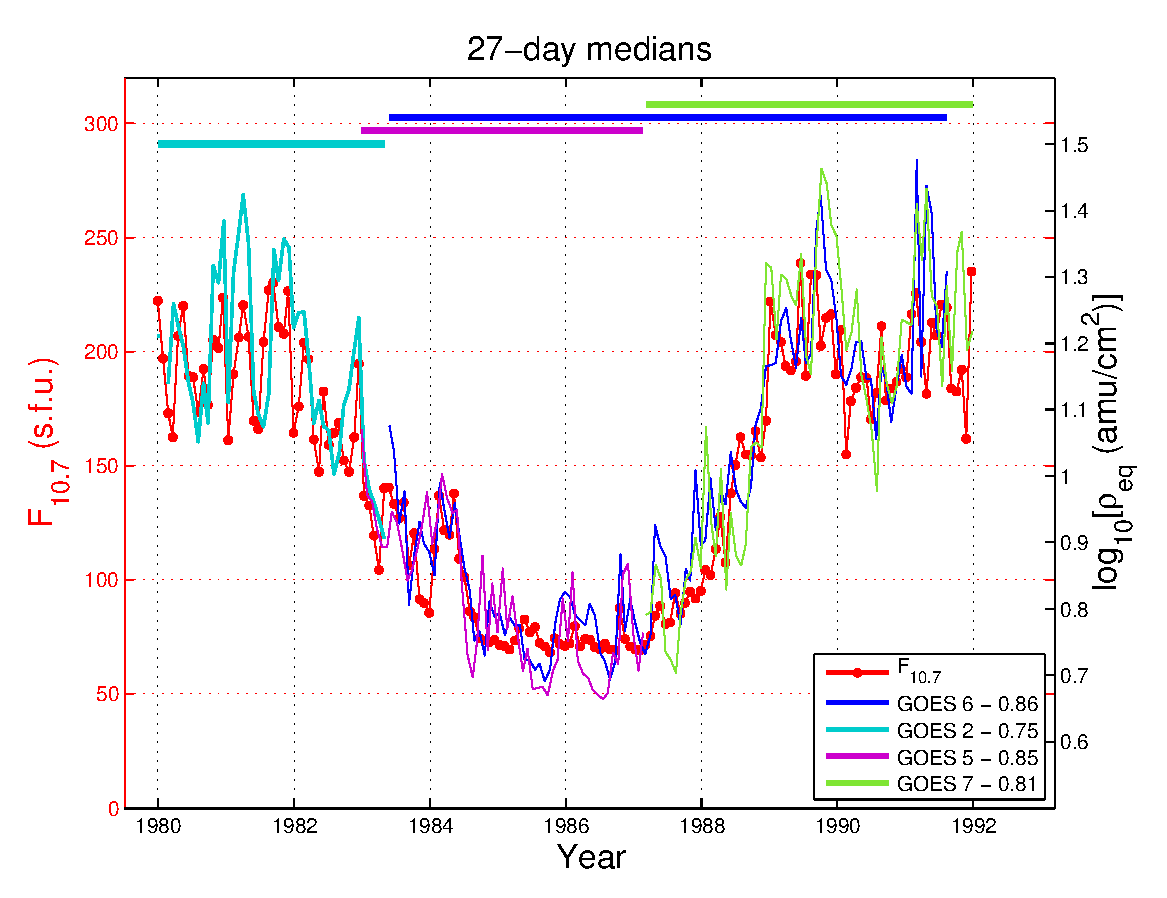
\includegraphics[width=0.95\linewidth]{Figures/F107MD27d-all}
	\caption{Comparing $F_{10.7\_27d}$ and $\log_{10}(\rho_{eq\_27d})$ using all available satellites.}
	\label{fig:F107rhoeq27dcomparison}
\end{figure}
\end{frame}


\subsection{Neural Network}
\begin{frame}
	\subheader
	 \begin{table}[h]
	 	\footnotesize
	 	\begin{tabular}{|C|CCCC|}
	 		\hline
	 		& \text{GOES 2} & \text{GOES 5} & \text{GOES 6} & \text{GOES 7}\\ \hline
	 		DoY & +0.05\pm0.31 & +0.31\pm0.30 & +0.32\pm0.22 & +0.12\pm0.17 \\
	 		MLT & +0.29\pm0.41 & +0.15\pm0.34 & +0.40\pm0.32 & +0.17\pm0.21 \\
	 		B_z & +0.24\pm0.23 & +0.21\pm0.28 & +0.17\pm0.19 & -0.00\pm0.20 \\
	 		V_{sw} & +0.20\pm0.25 & +0.36\pm0.19 & +0.19\pm0.24 & +0.06\pm0.18 \\
	 		D_{st} & +0.08\pm0.27 & +0.18\pm0.25 & +0.02\pm0.17 & +0.18\pm0.24 \\
	 		\rho_{sw} & +0.02\pm0.29 & +0.25\pm0.42 & +0.20\pm0.22 & +0.12\pm0.29 \\
	 		F_{10.7} & +0.26\pm0.27 & +0.32\pm0.29 & +0.48\pm0.25 & +0.36\pm0.15 \\
	 		B_z+V_{sw} & +0.11\pm0.25 & +0.20\pm0.38 & +0.15\pm0.21 & +0.02\pm0.17 \\
	 		D_{st}+F_{10.7} & +0.17\pm0.25 & +0.21\pm0.32 & +0.47\pm0.15 & +0.35\pm0.17 \\
	 		All & +0.21\pm0.41 & +0.67\pm0.40 & +0.60\pm0.35 & +0.17\pm0.33 \\
	 		\hline
	 	\end{tabular}
		\caption{Table of nonlinear model test correlations showing the median of 100 random samples. Each sample trained on half of the data (via randomly selected rows of the least squares matrix) and tested on the other half.} 
	 	\label{NNperltable}
	 \end{table}
\end{frame}


\subsection{Epoch}

\begin{frame}
	\subheader
	Epoch Analysis performed on two types of events:
	\begin{itemize}
		\item $\req >$ 20 amu/cm$^3$
		\item $\dst <$ -40 nT
	\end{itemize}
	Threshold crossings for events considered at an hourly timescale. First wanted to verify results of Takahashi (2010), looking at \dst\ events from 1989-1991 hitting a minimum between 06-12 MLT.
\end{frame}

\begin{frame}
	\begin{figure}[htp!]
		\centering
		\includegraphics[width=0.3\linewidth]{Figures/StormAvs/stormavs-Takahashi.png}
		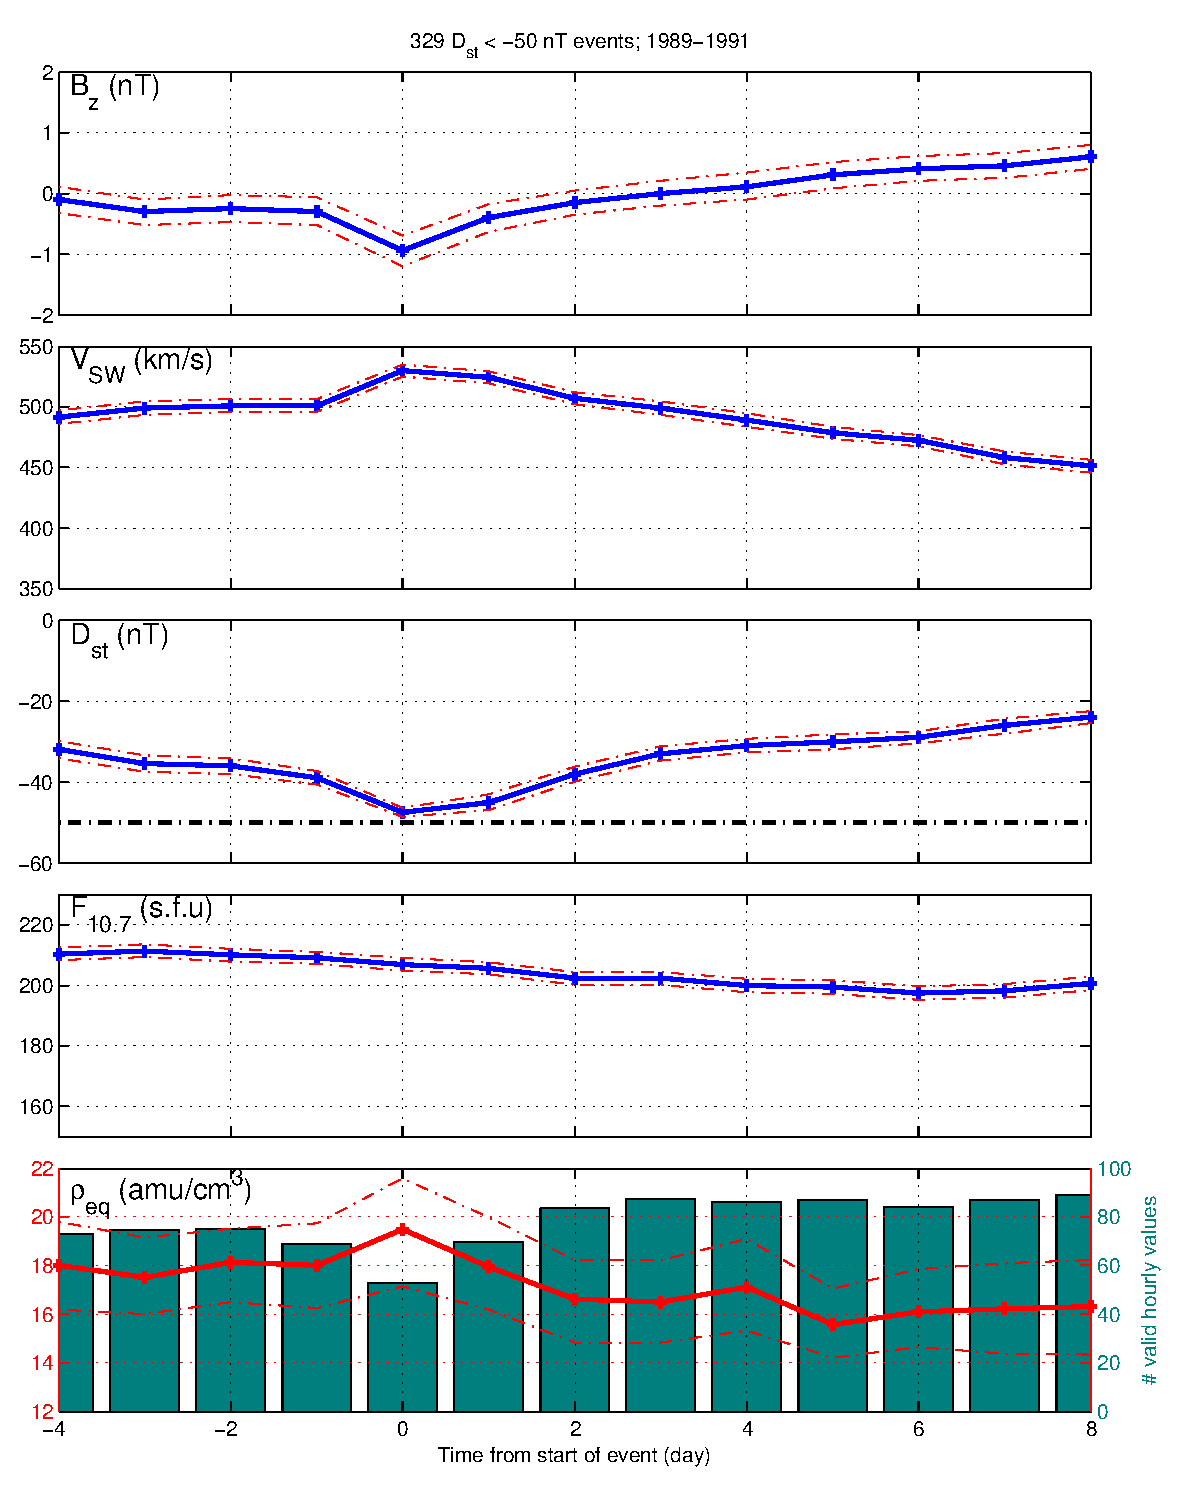
\includegraphics[width=0.45\linewidth]{Figures/StormAvs/stormavs-dst-50-tak-GOES6}
		\caption{Epoch analysis for \dst\ events on an daily timescale using only the years of 1989-1991 from Takahashi (2010).}
		\label{fig:EpochTakahashi}
	\end{figure}
\end{frame}

\begin{frame}
	To verify whether events were significantly different between day of onset and the surrounding days, a bootstrap test of differences was performed:
	\begin{figure}[htp!]
		\centering
		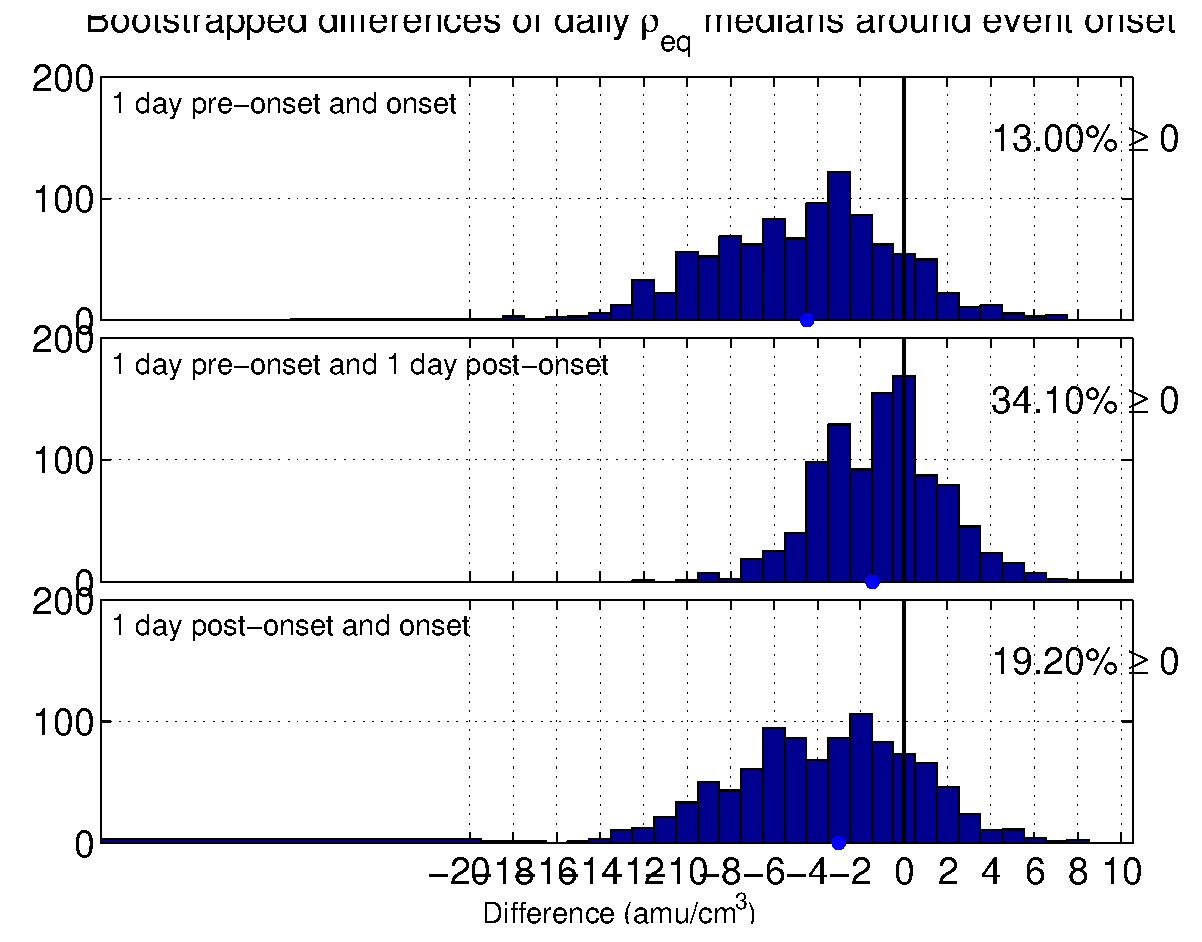
\includegraphics[width=0.6\linewidth]{Figures/DailyBootstrapDifferences-GOES6-case10}
		\caption{Bootstrap differences between median daily value of events using only the years of 1989-1991.}
		\label{fig:DailyBootstrapDifferences}
	\end{figure}
\end{frame}

\begin{frame}
	Using all of GOES 6's 1983-1991 range instead:
	\begin{figure}[htp!]
		\centering
		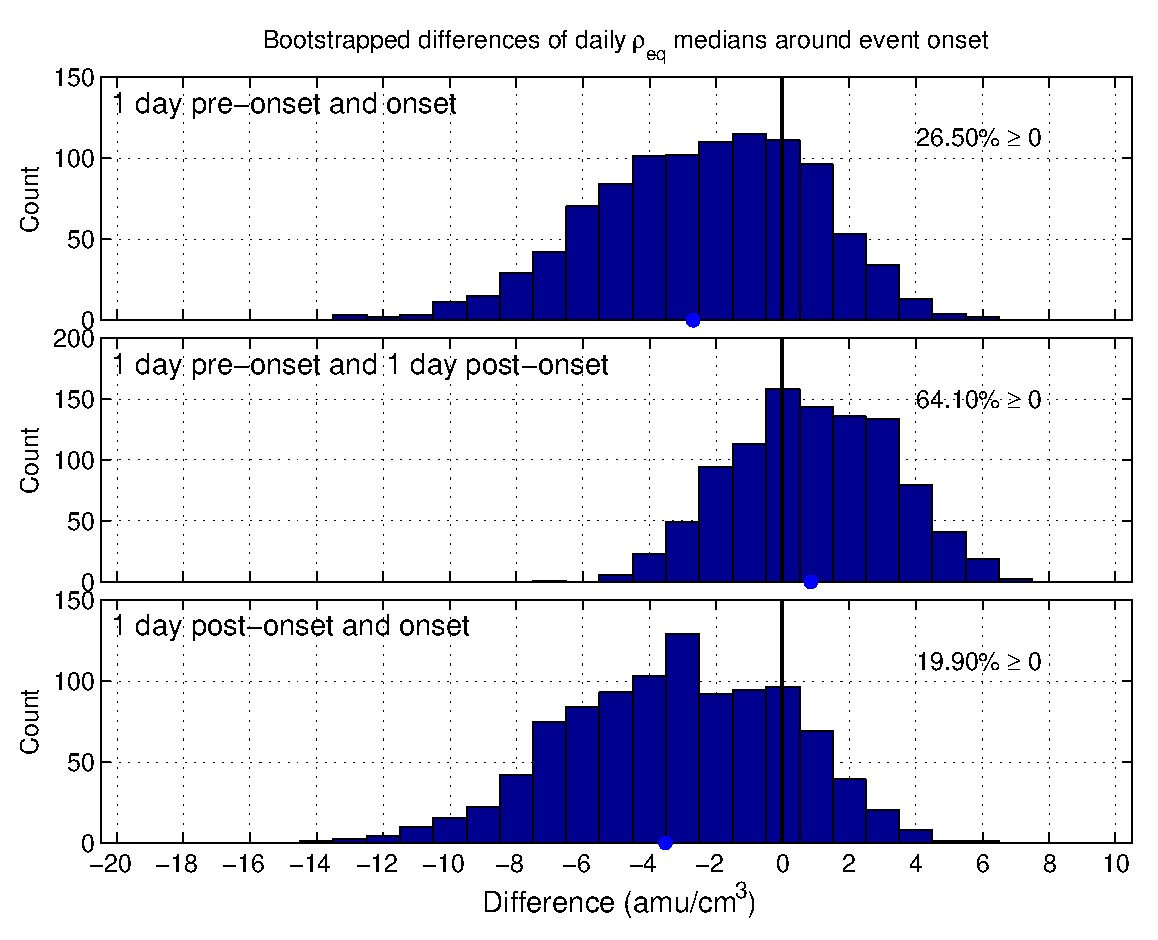
\includegraphics[width=0.6\linewidth]{Figures/DailyBootstrapDifferences-GOES6-case13}
		\caption{Bootstrap differences between median daily value of events using the years of 1983-1991.}
		\label{fig:DailyBootstrapDifferences-full}
	\end{figure}
\end{frame}



\begin{frame}
	\begin{figure}[htp!]
		\centering
		\includegraphics[width=0.5\linewidth]{Figures/StormAvs/stormavs-dst}
		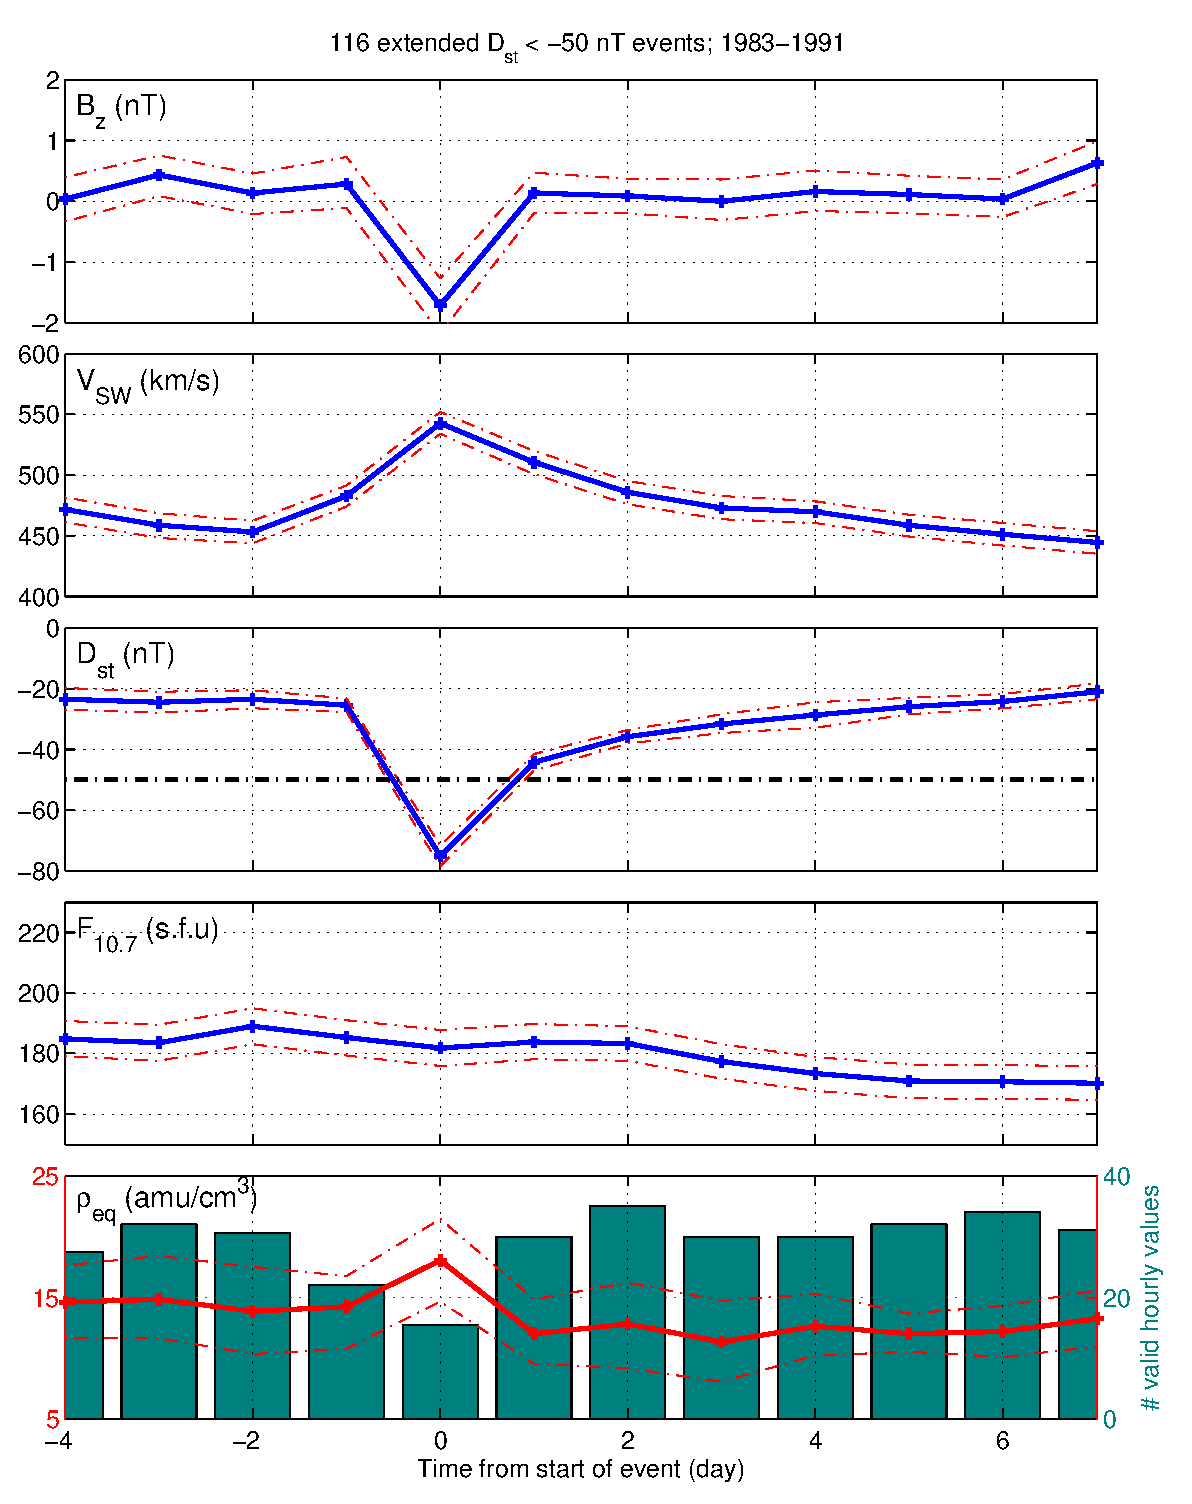
\includegraphics[width=0.5\linewidth]{Figures/StormAvs/stormavs-dst-day-GOES6}
		\caption{\dst\ events on an hourly (left) and daily (right) timescale.}
		\label{fig:EpochDst}
	\end{figure}
\end{frame}


\begin{frame}
\begin{figure}[htp!]
	\centering
	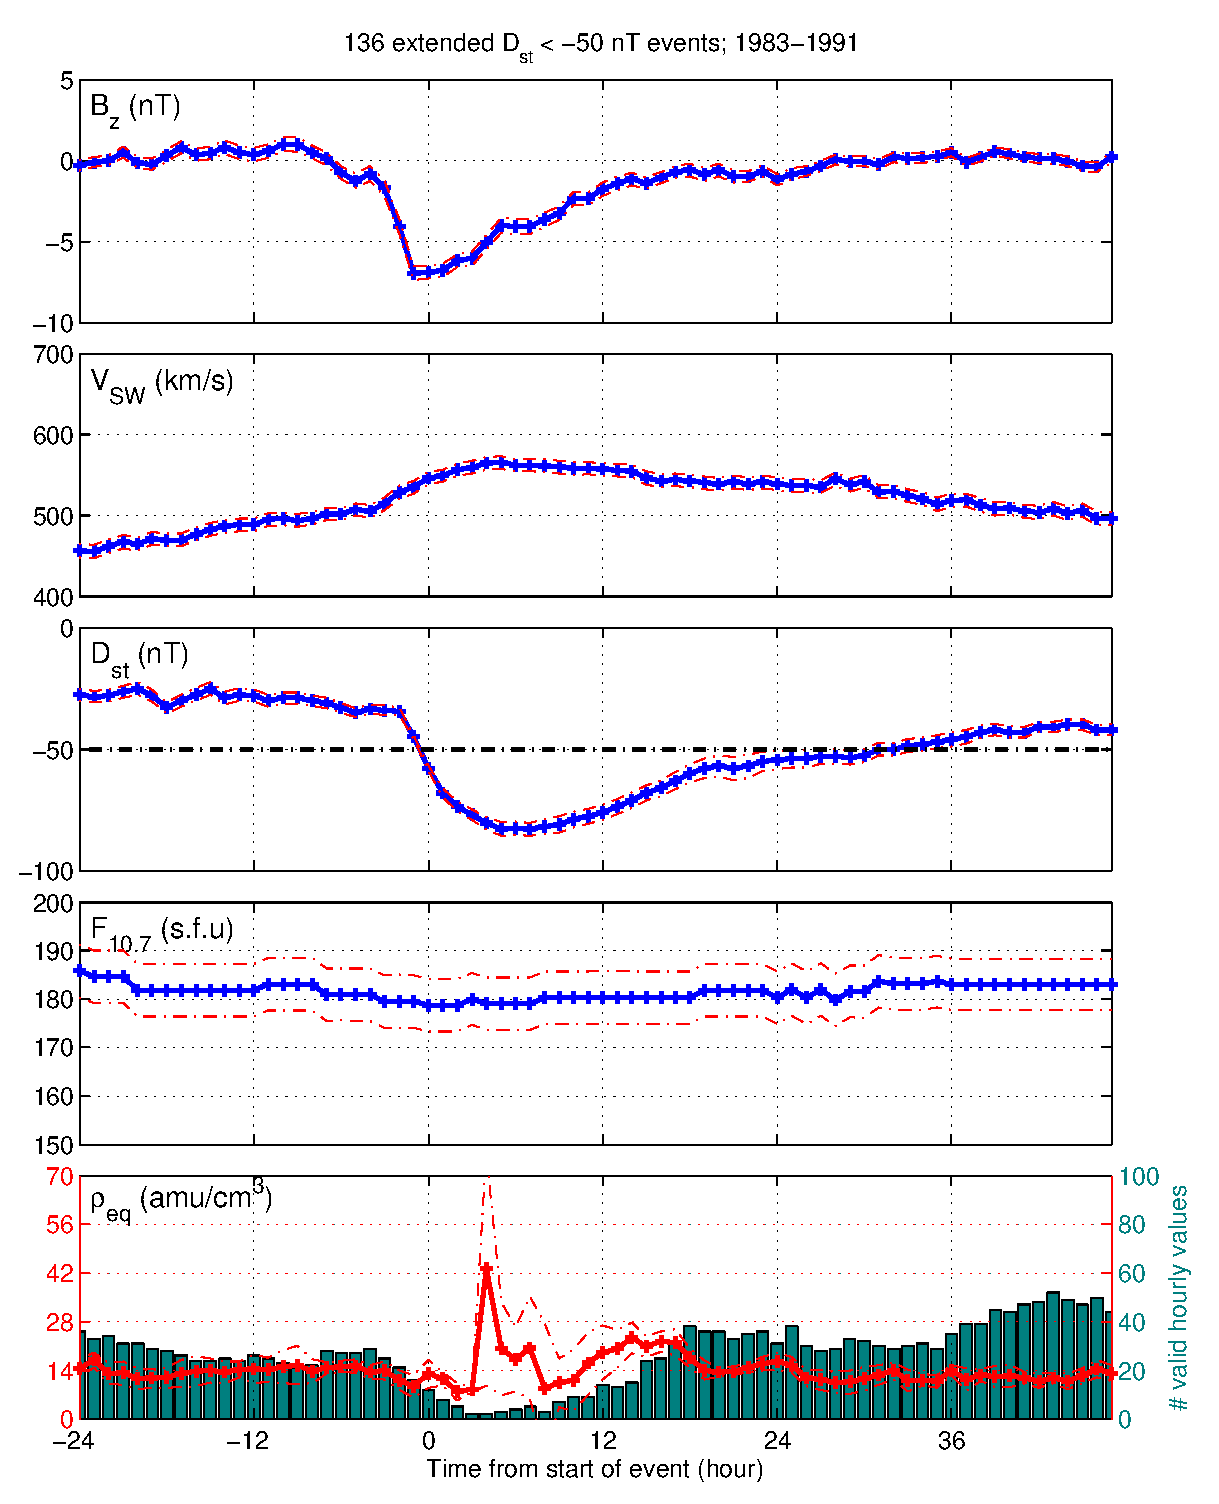
\includegraphics[width=0.4\linewidth]{Figures/StormAvs/stormavs-dd12-GOES6}
	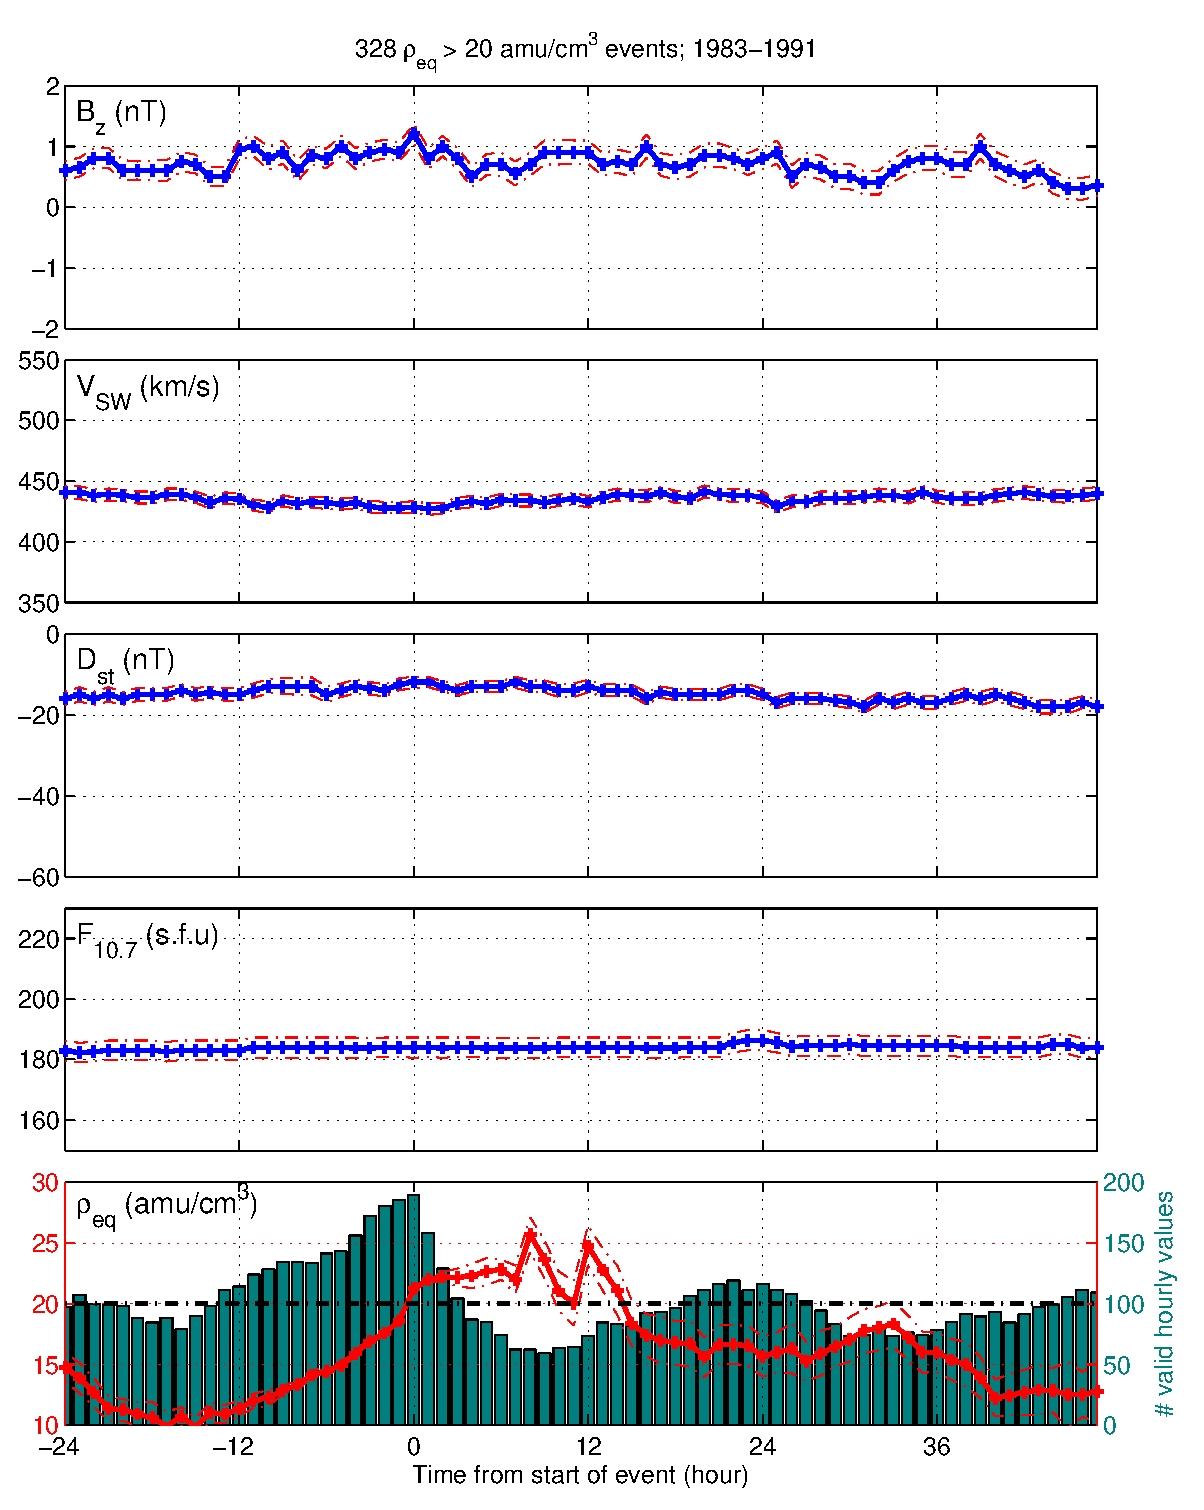
\includegraphics[width=0.4\linewidth]{Figures/StormAvs/stormavs-mass-gt20-GOES6}
	\caption{Left: \dst\ events lasting longer than 12 hours. Right: \req\ events on hourly timescale.}
	\label{fig:EpochDst12Hour}
\end{figure}
\end{frame}


\begin{frame}
	Want to investigate nonlinear dependencies by binning events:
	\begin{figure}[htp!]
		\centering
		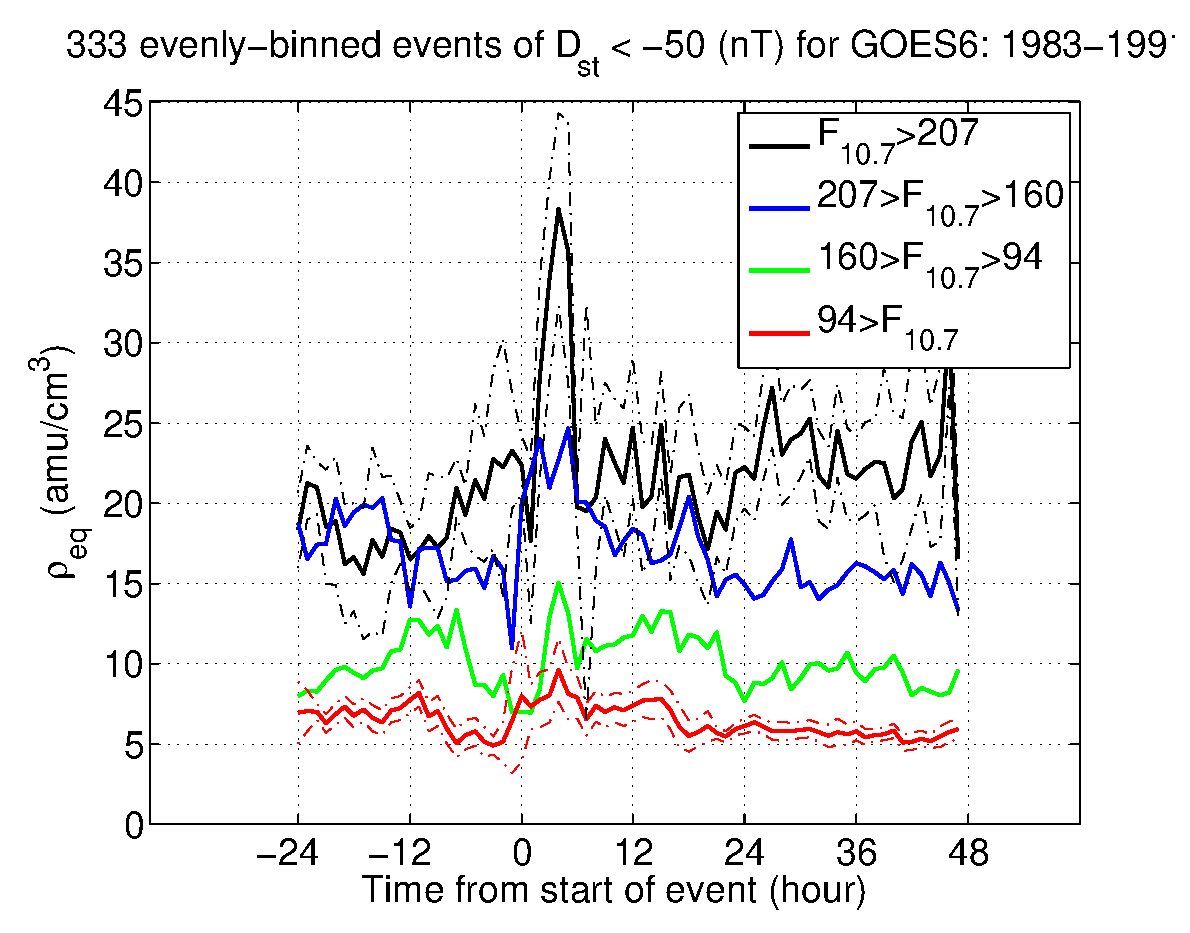
\includegraphics[width=0.5\linewidth]{Figures/HighLowF107rhoeq-Dst50-GOES6-1983-1991}
		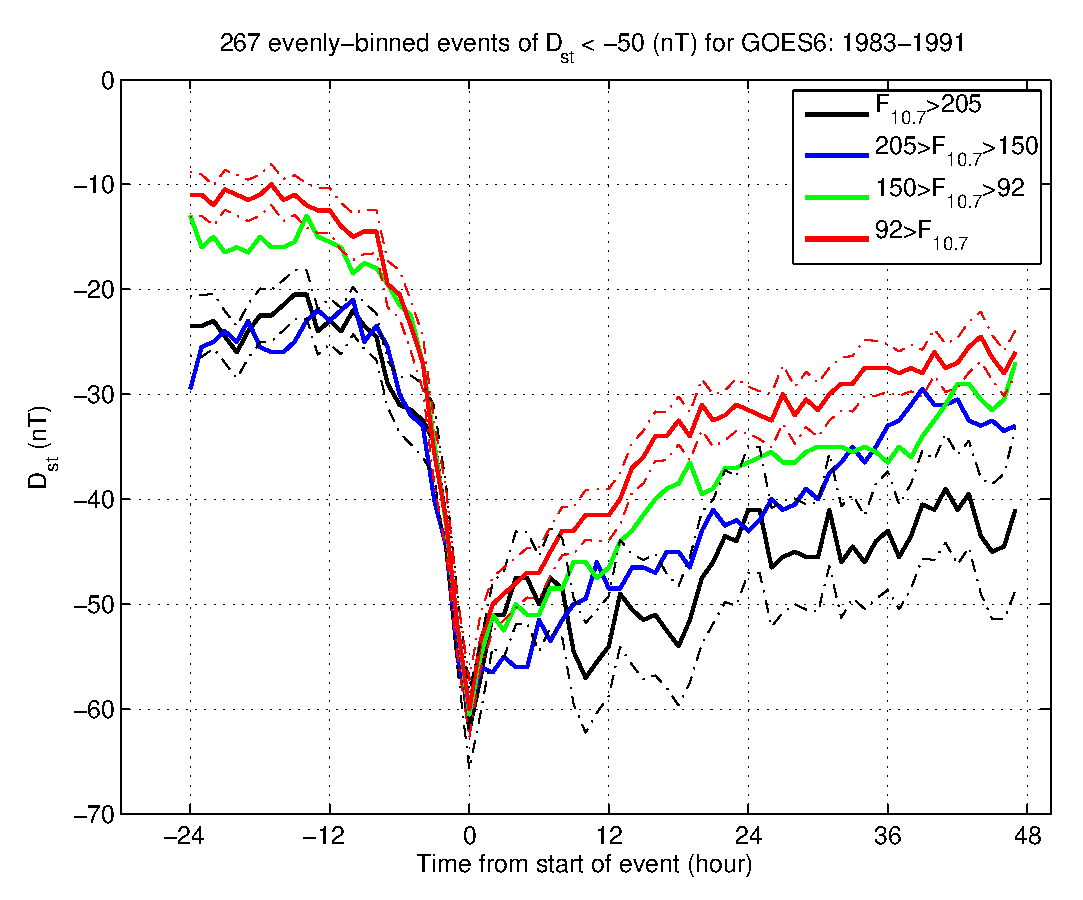
\includegraphics[width=0.5\linewidth]{Figures/HighLowF107Dst-Dst50-GOES6-1983-1991}	
		\caption{\req\ (left) and \dst\ (right) of \dst\ events binned by median \f\ values.}
		\label{fig:HighLowF107rhoeq}
	\end{figure}
\end{frame}

\begin{frame}
	Verifying that distribution of \req\ is significantly different per \f\ bin before and after \req\ event onset.
	\begin{figure}[htp!]
		\centering
		\includegraphics[width=0.5\linewidth]{Figures/RhoBinnedF_{10.7}-case24-t020-tf25-GOES6}
		\includegraphics[width=0.5\linewidth]{Figures/RhoBinnedF_{10.7}-case24-t025-tf30-GOES6}	
		\caption{\req\ events binned by median \f\ before (left) and after (right) event onset.}
		\label{fig:RhoBinnedF107}
	\end{figure}
\end{frame}

\begin{frame}
	Verifying that distribution of \req\ is also significantly different per \f\ bin before and after \dst\ event onset.
	\begin{figure}[htp!]
		\centering
		\includegraphics[width=0.5\linewidth]{Figures/RhoBinnedF_{10.7}-case1-t020-tf25-GOES6}
		\includegraphics[width=0.5\linewidth]{Figures/RhoBinnedF_{10.7}-case1-t025-tf30-GOES6}	
		\caption{\dst\ events binned by median \f\ before (left) and after (right) event onset.}
		\label{fig:RhoBinnedF107}
	\end{figure}
\end{frame}

%%%%%%%%%%%%%%%%%%%%%%%%%%%%%%%%%%%%%%%%%%%%%%%%%%%
%  _____                  _           _                 
% /  __ \                | |         (_)                
% | /  \/ ___  _ __   ___| |_   _ ___ _  ___  _ __  ___ 
% | |    / _ \| '_ \ / __| | | | / __| |/ _ \| '_ \/ __|
% | \__/| (_) | | | | (__| | |_| \__ | | (_) | | | \__ \
% \_____/\___/|_| |_|\___|_|\__,_|___|_|\___/|_| |_|___/
%%%%%%%%%%%%%%%%%%%%%%%%%%%%%%%%%%%%%%%%%%%%%%%%%%%
\section{Conclusions}



\subsection{Future work}
\begin{frame}
	Many things could be done to improve:
	\begin{itemize}
		\item Find new description of Lax-Wendroff scheme to check for inconsistencies
		\item Try higher order finite-difference scheme for derivatives
		\item Start from steady state magnetosphere
		\item Attempt 3D simulation
		\item Use non-discontinuous near-Earth model without fixed state
	\end{itemize}
\end{frame}

\begin{frame}[c]
	\begin{center}
		\huge
		Questions?
	\end{center}
	\small
	\begin{itemize}
		\item Do I need to explain F10.7? How about geomagnetic indices, and to what depth?
		\item References page? Fine to fill out by hand?
		\item Too many tables? Fine to drop extra satellites to fit L, ARX, and NL on one slide?
	\end{itemize}
\end{frame}





\begin{frame}
	\tiny
	\bibliographystyle{plainnat-lastnamefirst}
	\bibliography{bibfile}
\end{frame}





\end{document}